\documentclass[letterpaper, oneside]{book}

\usepackage{tree-dvips}
\usepackage{amsmath}
\usepackage{listings}
\usepackage{graphicx}
\usepackage{xcolor}
\usepackage{mdframed}
\usepackage{fancyhdr}
\usepackage[export]{adjustbox}
\usepackage[skip=10pt]{parskip}
\usepackage{amsfonts}
\usepackage{hyperref}
\usepackage{algorithm}
\usepackage{algpseudocode}
\pagestyle{plain}

% Configure listings backage for code
\lstset{
    %numbers=left,
    %numberstyle=\tiny,
    breaklines=true,
    %numbersep=5pt,
    xleftmargin=.45in,
    xrightmargin=.05in}

\graphicspath{{./resources/}}


\title{System Design Notes}
\author{Ryan}
\date{July 2024}

\begin{document}

\maketitle{}
\tableofcontents


%%%%%%%%%%%%%%%%%%%%%%%%%%%%%%%%%%%%%%%%%%%%%%%%%%%%
%%%%%%%%%%%%%%%%%%%%%%%%%%%%%%%%%%%%%%%%%%%%%%%%%%%%
\part{Common Knowledge}


%%%%%%%%%%%%%%%%%%%%%%%%%%%%%%%%%%%%%%%%%%%%%%%%%%%%
\chapter{Keywords}
%%%%%%%%%%%%%%%%%%%%%%%%%%%%%%%%%%%%%%%%%%%%%%%%%%%%

DNS; monolithic; tiered architecture; database management system; relational database; vertical scaling; horizontal scaling; failover; redundancy; load balancer; database replication; cache; eviction policy; expiration policy; consistent hashing; cache miss; cache hit; caching strategy; single point of failure; stateful webserver; stateless webserver; CDN; message queue; normalization; de-normalization; sharding; rate limiting; optimistic lock; eventual consistency; transaction log; lease; fan-out; rollback

%%%%%%%%%%%%%%%%%%%%%%%%%%%%%%%%%%%%%%%%%%%%%%%%%%%%
%%%%%%%%%%%%%%%%%%%%%%%%%%%%%%%%%%%%%%%%%%%%%%%%%%%%
\part{Fundamentals and Building Blocks}



%%%%%%%%%%%%%%%%%%%%%%%%%%%%%%%%%%%%%%%%%%%%%%%%%%%%
\chapter{Consistent Hashing}
%%%%%%%%%%%%%%%%%%%%%%%%%%%%%%%%%%%%%%%%%%%%%%%%%%%%

%%%%%%%%%%%%%%%%%%%%%%%%%%%%%%%%%%%%%%%%%%%%%%%%%%%%
\chapter{Cache}
%%%%%%%%%%%%%%%%%%%%%%%%%%%%%%%%%%%%%%%%%%%%%%%%%%%%

caching strategy; expiration policy; eviction policy; invalidation

Caches and cache layers are key components in almost every high-performance architecture. The idea is to save results that are expensive to obtain. Examples are prediction calculated by a complex machine learning algorithms or data extracted from a database.

When employing caches, it's important to remember two important characteristics of caches:
\begin{itemize}
    \item It requires additional efforts to maintain the consistency between caches and the authoritative source of the data.
    \item Caches are ephemeral. When designing a system that uses caches, we need to assume we could lose the cached items at anytime.
\end{itemize}

\section{Distributed Cache}


%%%%%%%%%%%%%%%%%%%%%%%%%%%%%%%%%%%%%%%%%%%%%%%%%%%%
\chapter{Lock}
%%%%%%%%%%%%%%%%%%%%%%%%%%%%%%%%%%%%%%%%%%%%%%%%%%%%

\subsection{Default Locking}

\subsection{Optimistic Locking}

\subsection{Distributed Locks}

%%%%%%%%%%%%%%%%%%%%%%%%%%%%%%%%%%%%%%%%%%%%%%%%%%%%
\chapter{Message Queue}
%%%%%%%%%%%%%%%%%%%%%%%%%%%%%%%%%%%%%%%%%%%%%%%%%%%%


%%%%%%%%%%%%%%%%%%%%%%%%%%%%%%%%%%%%%%%%%%%%%%%%%%%%
\chapter{Design Patterns}
%%%%%%%%%%%%%%%%%%%%%%%%%%%%%%%%%%%%%%%%%%%%%%%%%%%%

\section{Partition}
Partition or sharding is a direct application of the divide-and-conquer strategy. Instead of routing all the work to a single machine, we distribute the work to a cluster of machines. Partitioning the workload is a crutial step if we want to horizontally scale the system. The partitioning implementation needs to take into account the fact the size of cluster may change.
For example, during a cluster maintenance, some machines may be shutdown, resulting in a decrease of the cluster capacity. Or we may need to add more machines to accommodate an increase in the request load. When the cluster size changes, requests may be routed to a different machines, which may not be ready to process the request efficiently. A typical solution to this problem is consistent hashing.


\section{Leader Follower Pattern}




%%%%%%%%%%%%%%%%%%%%%%%%%%%%%%%%%%%%%%%%%%%%%%%%%%%%
\chapter{Classic Architecture}
%%%%%%%%%%%%%%%%%%%%%%%%%%%%%%%%%%%%%%%%%%%%%%%%%%%%

\section{Basic Template}

The diagram below demonstrates one of the basic structures of application services. Uses, such as mobile devices or applications running on servers send request to the endpoint of the target services. When the user request enters the service boundary, it usually hits a load balancer first. The load balancer is responsible for evenly distribute use requests to application servers in the cluster. The

For application servers form a cluster, there is usually a piece of code responsible for coordination. Servers may play different roles in a cluster, for example, some of the servers are coordinators and others are workers.



\begin{figure}[h]
    \centering
    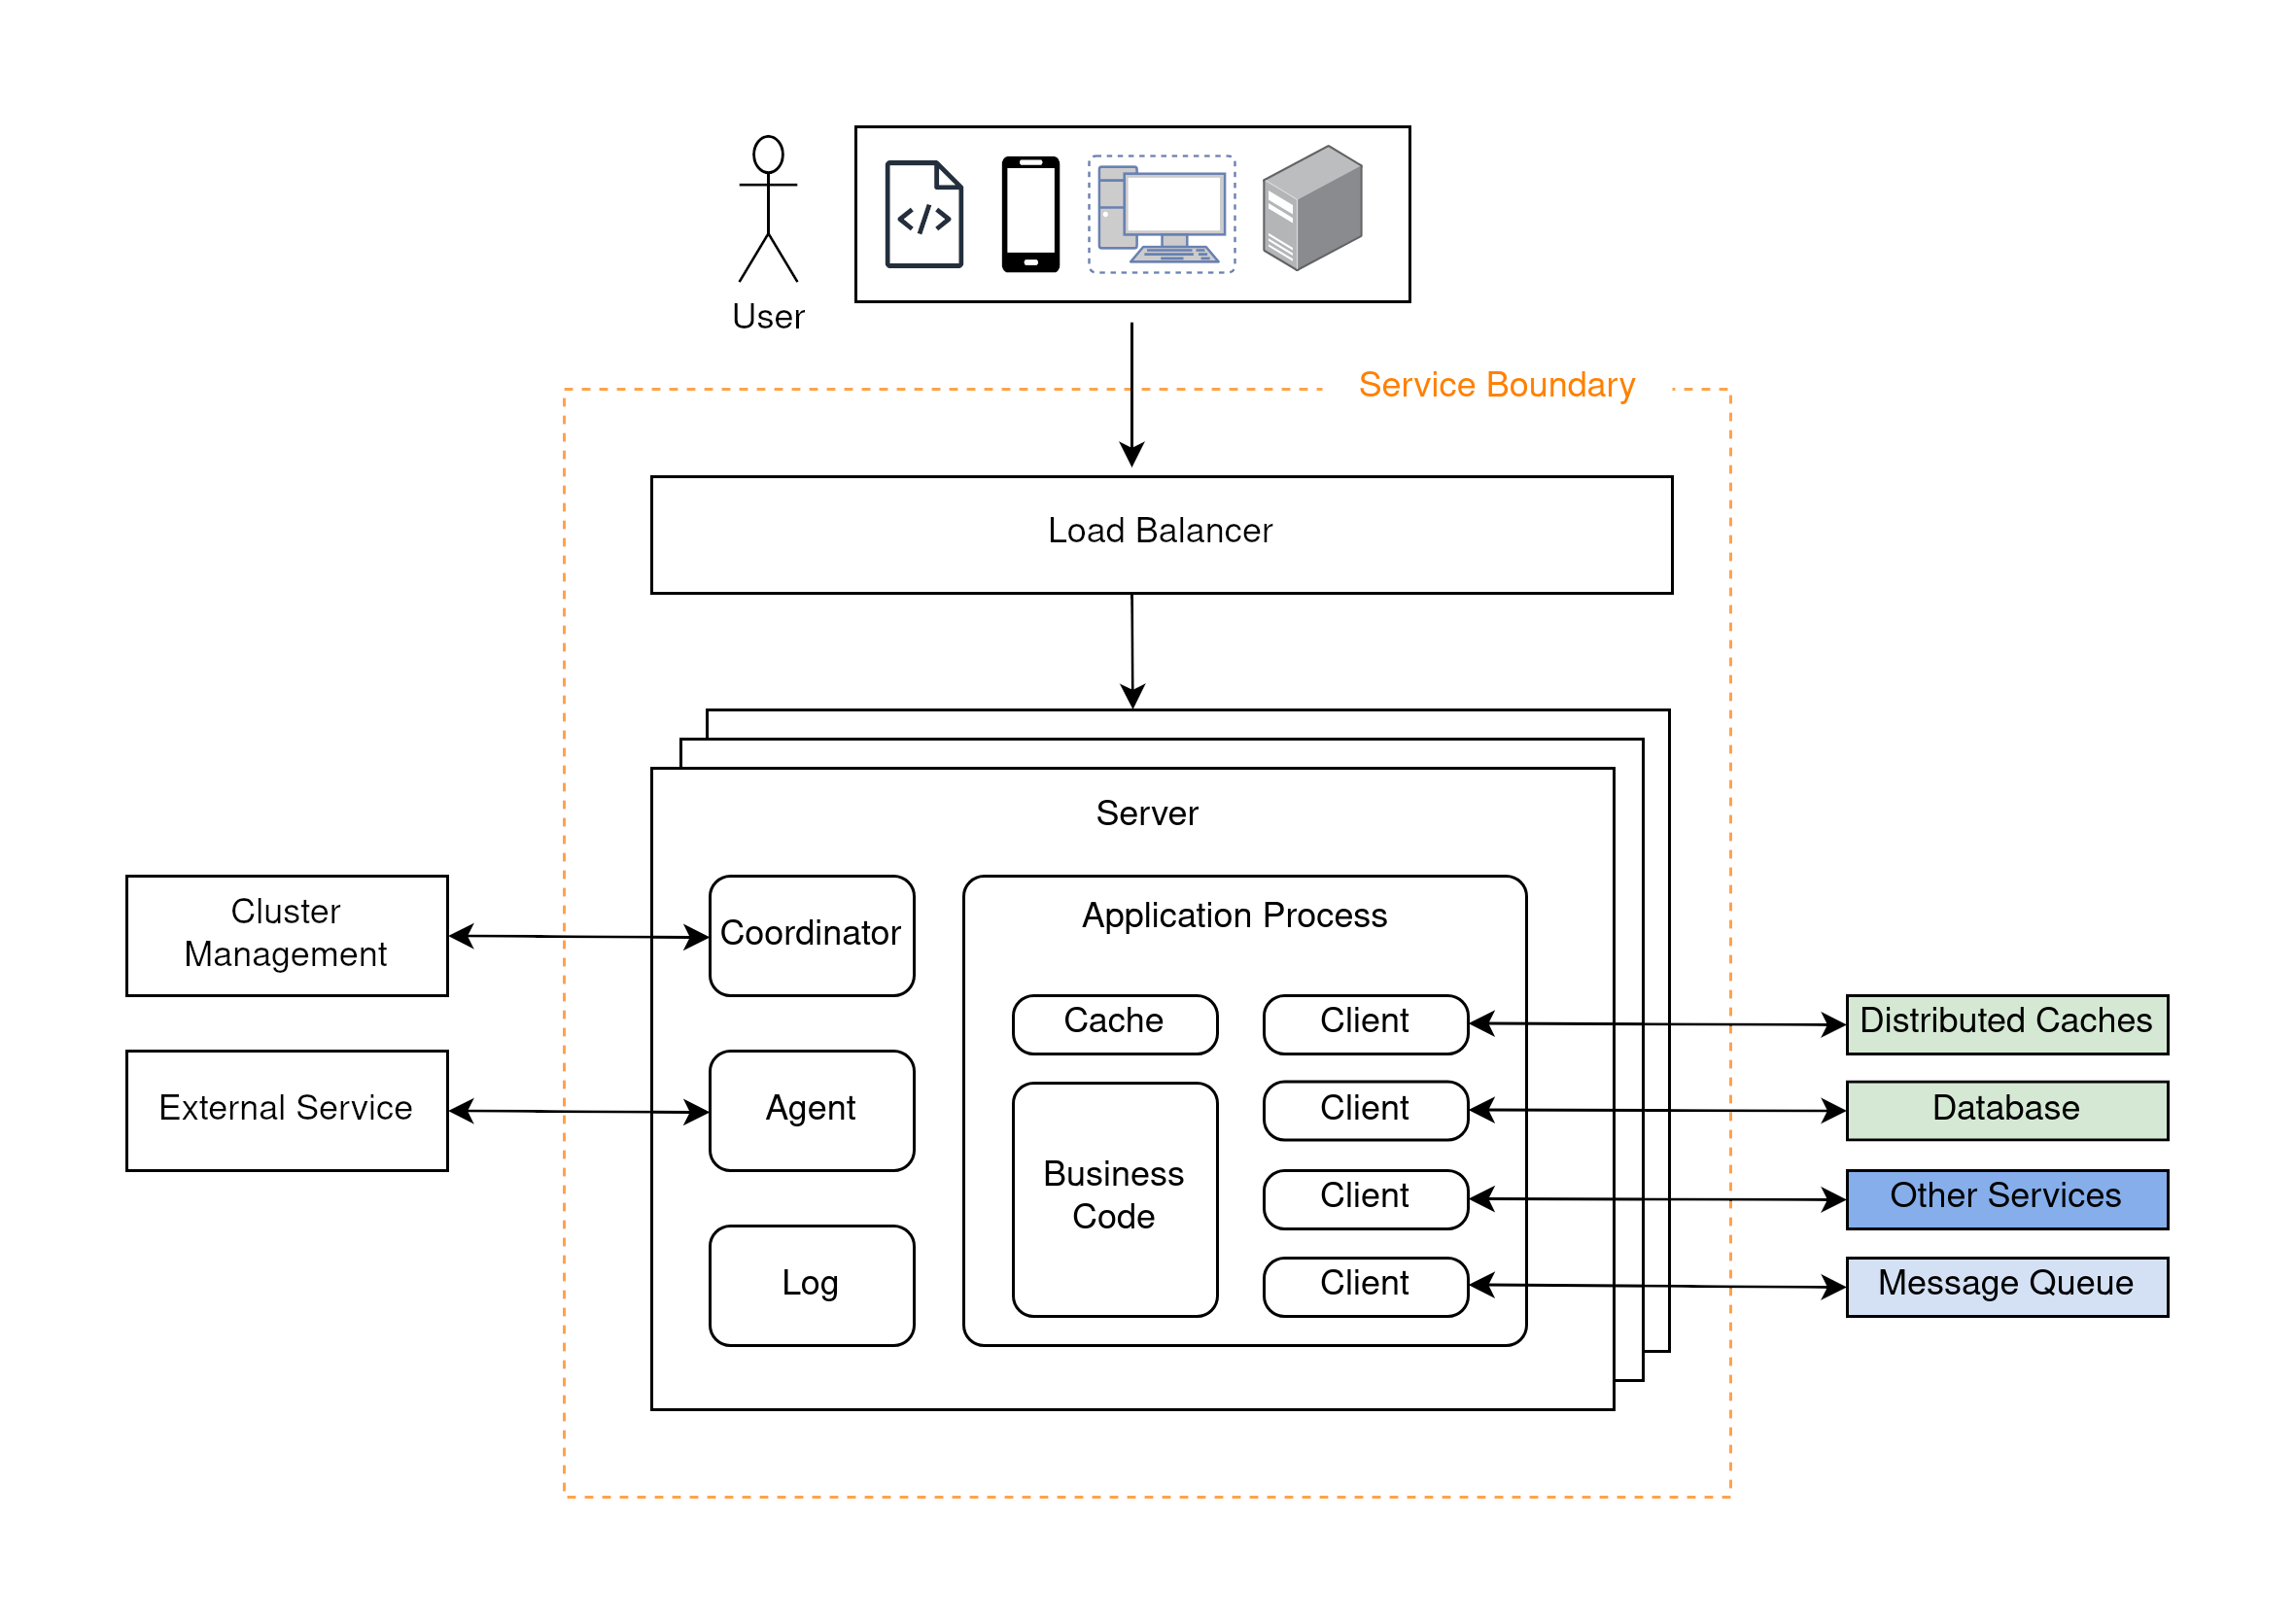
\includegraphics[width=0.90\textwidth]{system_design_basic_template.png}
    \caption{A basic template}
    \label{fig:basic_template}
\end{figure}


%%%%%%%%%%%%%%%%%%%%%%%%%%%%%%%%%%%%%%%%%%%%%%%%%%%%
\chapter{Data Modeling}
%%%%%%%%%%%%%%%%%%%%%%%%%%%%%%%%%%%%%%%%%%%%%%%%%%%%
normalization; denormalization


%%%%%%%%%%%%%%%%%%%%%%%%%%%%%%%%%%%%%%%%%%%%%%%%%%%%
%%%%%%%%%%%%%%%%%%%%%%%%%%%%%%%%%%%%%%%%%%%%%%%%%%%%
\part{Cloud Technology}

%%%%%%%%%%%%%%%%%%%%%%%%%%%%%%%%%%%%%%%%%%%%%%%%%%%%
\chapter{AWS}
%%%%%%%%%%%%%%%%%%%%%%%%%%%%%%%%%%%%%%%%%%%%%%%%%%%%


\part{Database}

%%%%%%%%%%%%%%%%%%%%%%%%%%%%%%%%%%%%%%%%%%%%%%%%%%%%
\chapter{Relational Database}
%%%%%%%%%%%%%%%%%%%%%%%%%%%%%%%%%%%%%%%%%%%%%%%%%%%%
transaction log; commit log;


%%%%%%%%%%%%%%%%%%%%%%%%%%%%%%%%%%%%%%%%%%%%%%%%%%%%
\chapter{Non-relational Database}
%%%%%%%%%%%%%%%%%%%%%%%%%%%%%%%%%%%%%%%%%%%%%%%%%%%%

Non-relational databases might be the right choice if:
\begin{itemize}
    \item Your application requires super-low latency.
    \item Your data are unstructured, or you do not have any relational data.
    \item You only need to serizliae and deserialize data.
    \item You need to store a massive amount of data.
\end{itemize}






\end{document}
